\section{Description of the user interface}\label{interface} 
The graphical user interface is very easy to use. An example is given in Figure~\ref{ui} (p. \pageref{ui}) how the interface looks like. 

\begin{figure}
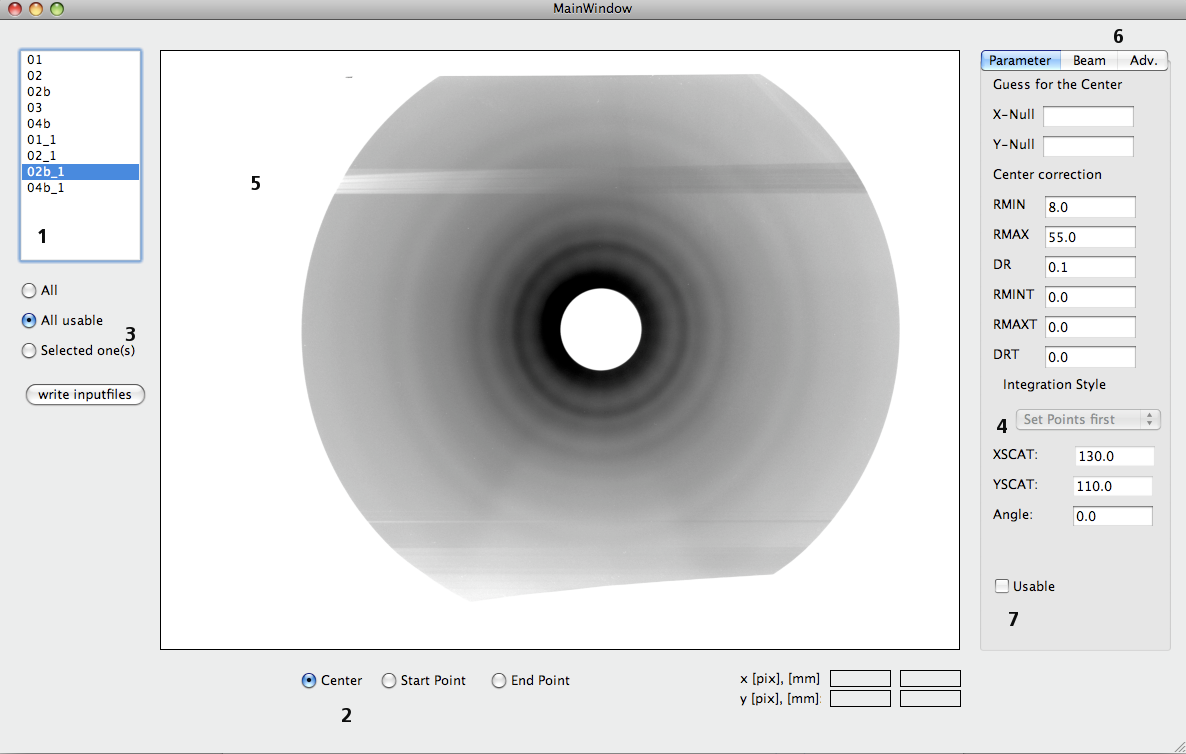
\includegraphics[width=20cm, angle=90]{ui.png}
\caption{Typical screenshot of the user interface. (1) The itemlist (listWidget), (2) Radiobuttons for selecting points, (3) Radiobuttons for selecting which input files to write out, (4) drop-down menu for selecting data reduction style, (5) main graphic, (6) tabs to set more parameters and (7) the usable checkbox. }
\label{ui} 
\end{figure} 

\subsection{Input}
The program can deal with all kind of image formats. It was tested with .tif files but should work with all other formats, as long as they are supported by Qt. \\
The the images can be opened with the OpenFile menu. \\
The following should be considered:
\begin{enumerate}
\item The program assumes that the data files (.img) are in the same directory then the image files (.tif). 
\item The pimag executable must be in the same directory then the .tif and .img files. Otherwise the data reduction (see later) will not work. 
\end{enumerate}

\subsection{Workflow}
A complete workflow is described in Figure~\ref{workflow} (p. \pageref{workflow}). The workflow describes one way to work with the program. Theoretically it is possible to go back at any point of the diagram. 

\begin{figure}
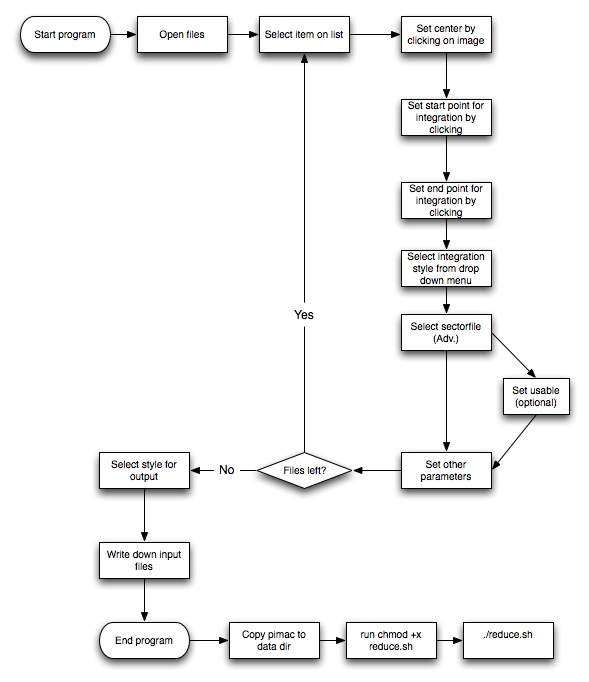
\includegraphics[width=12cm]{diagram}
\caption{Workflow of the program.The "set usable"-step is optional, depending on the way the input files are written out later. If you decide to write out input files for every image, it is not necessary to set.  }
\label{workflow} 
\end{figure} 

\subsection{Output}
The program hast tree modes to write out input files for pimag. For all images imported, for all images selected in the list or for all images flagged as usable. \\
For every image one .txt file is written out to the same directory then the image files. \\
In the end a bash-script is written do reduce.sh that can be used for data reduction. Notice that it must be executable (chmod +x) to execute it. Assuming the .tif and .img files are in /home/geduser/mydata/, the following has to be done: \\

\begin{lstlisting}
cd /home/geduser/mydata/
chmod +x reduce.sh
./reduce.sh 
\end{lstlisting}

The last command starts the data reduction. The script creates (or overrides!) the following files, assuming that \$filename was the name of the .tif file, without the .tif.  

\begin{itemize}
\item [\$filename.curv] This file is used for further processing of the data. 
\item [\$filename.plot] This file is used for plotting, a free program like xmgr \cite{xmgr} or GNUPLOT \cite{gnuplot} can be used. 
\end{itemize}




